\documentclass[11pt,a4]{article}
\usepackage{graphicx}
\usepackage{xcolor}
\usepackage{tabularx}
\usepackage{amsmath}
\usepackage[utf8]{inputenc}
\usepackage[T1]{fontenc}
\usepackage[french]{babel}
\usepackage{hyperref}
\usepackage{pdfpages}
\pagestyle{empty}
\topmargin -2cm
\textheight 22cm
\textwidth 15 cm
\oddsidemargin 0.46cm
\evensidemargin 0.46cm
\parskip=0.2 true cm
\headsep 2.cm

\begin{document}

% en-tête

\begin{figure}
    \begin{minipage}[c]{.06\linewidth}
        
\includegraphics[width = 3.5 true cm]{../phast-logo.png}
    \end{minipage} \hfill
    \begin{minipage}[c]{.66\linewidth}
        \begin{center}
            {\bf \Large Campagne 2019 de recrutement \\ sur contrat doctoral}
        \end{center}
    \end{minipage}
    \begin{minipage}[c]{.06\linewidth}
        
\includegraphics[width = 3.5 true cm]{../UdL-logo.png}
    \end{minipage}
\end{figure}

\begin{center}
    {\bf \Large Dossier de candidature -- Partie A (CV académique)}
\end{center}

% Photo candidat

\begin{center}
    \begin{tabular}{|m{12cm}|m{4cm}|} \hline
    \vspace{1.5cm} {\hskip 5 true cm} \textsc{Nicolas} Nora \vspace{1.5cm}
    & \hspace{.7cm} 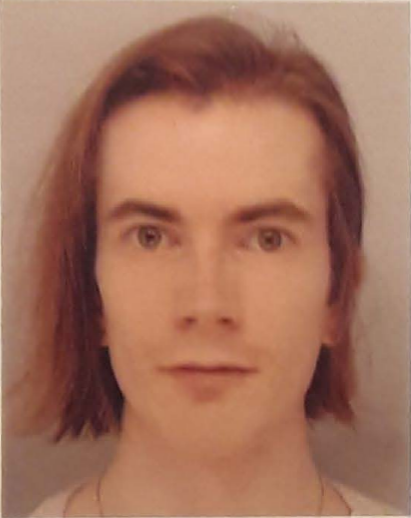
\includegraphics[width = 2 cm]{../nora_pid.png}
        \\ \hline
    \end{tabular}
\end{center}

% Informations

\noindent {\bf Adresse personnelle :} 
3 boulevard des Brotteaux, 69006 Lyon

\vglue 0.5 true cm

\noindent {\bf Téléphone portable :}
06 06 53 50 92

\vglue 0.5 true cm

\noindent {\bf Adresse électronique :}
\href{mailto:nora.nicolas@ens-lyon.fr}{nora.nicolas@ens-lyon.fr}

\vglue 0.5 true cm

\noindent {\bf Libellé du master :}
ENS de Lyon, Master Physique, Concepts et Applications

\vglue 0.5 true cm

\noindent {\bf Nom et adresse électronique du responsable pouvant attester du classement :}
\textsc{Bartolo} Denis, \href{mailto:denis.bartolo@ens-lyon.fr}{denis.bartolo@ens-lyon.fr}

\vglue 0.5 true cm

\noindent {\bf Cursus académique :} \\ Pour l'année universitaire en cours, seuls les résultats
partiels sont demandés.

\begin{center}
    \begin{tabular}{|c|c|c|c|c|c|} \cline{1-6}
        Année     & Formation               & Établissement & Moyenne & Rang & Effectifs \\ \hline
        2018-2019 & M2 Recherche            & ENS de Lyon   & 11.3    &      & 48 \\ \hline
        2017-2018 & M2 FEADéP -- Agrégation & ENS de Lyon   & 14.6    & 9    & 23 \\ \hline
        2016-2017 & M1 Recherche            & ENS de Lyon   & 12.5    & 56   & 61 \\ \hline
        2015-2016 & L3 Physique             & ENS de Lyon   & 15.6    & 19   & 50 \\ \hline
    \end{tabular}
\end{center}

\newpage
\noindent {\bf Lettre de motivation (max 15 lignes) :}\\

Étant actuellement en dernière année de mon cursus universitaire, je souhaite fortement continuer
mon parcours par une thèse en physique l'année prochaine. Je me suis intéressée à l'astrophysique et
la cosmologie dès le collège, sans pour autant m'y enfermer et en faire mon seul objectif ; c'est
ainsi qu'arrivée à l'ENS, j'ai continué mon exploration des différentes branches de la physique par
le biais de cours à la fois théoriques et pratiques, dont la cosmologie.

Mes stages ont toujours renouvelé mon engouement pour cette discipline, et ont été l'occasion de
mettre à profit mes connaissances, d'apprendre différents langages de programmation et d'être inclue
dans des projets de recherche conséquents. Ce furent de très bonnes expériences et j'ai ainsi pu
comprendre les attentes inhérentes à un travail de recherche sur le long terme, ainsi que la
nécessité de faire partie d'un groupe dynamique aux méthodes de travail rigoureuses.  J'ai été
charmée par ce sujet de thèse et la possibilité de manier à la fois théorie, étude de données et
observations, tout en traitant d'un sujet passionnant et au carrefour de nombreuses branches de la
recherche en physique.

La perspective de réaliser une thèse dans ce domaine est donc la concrétisation de mon parcours
riche en expériences et de ma préférence initiale.

\vglue 7 true cm

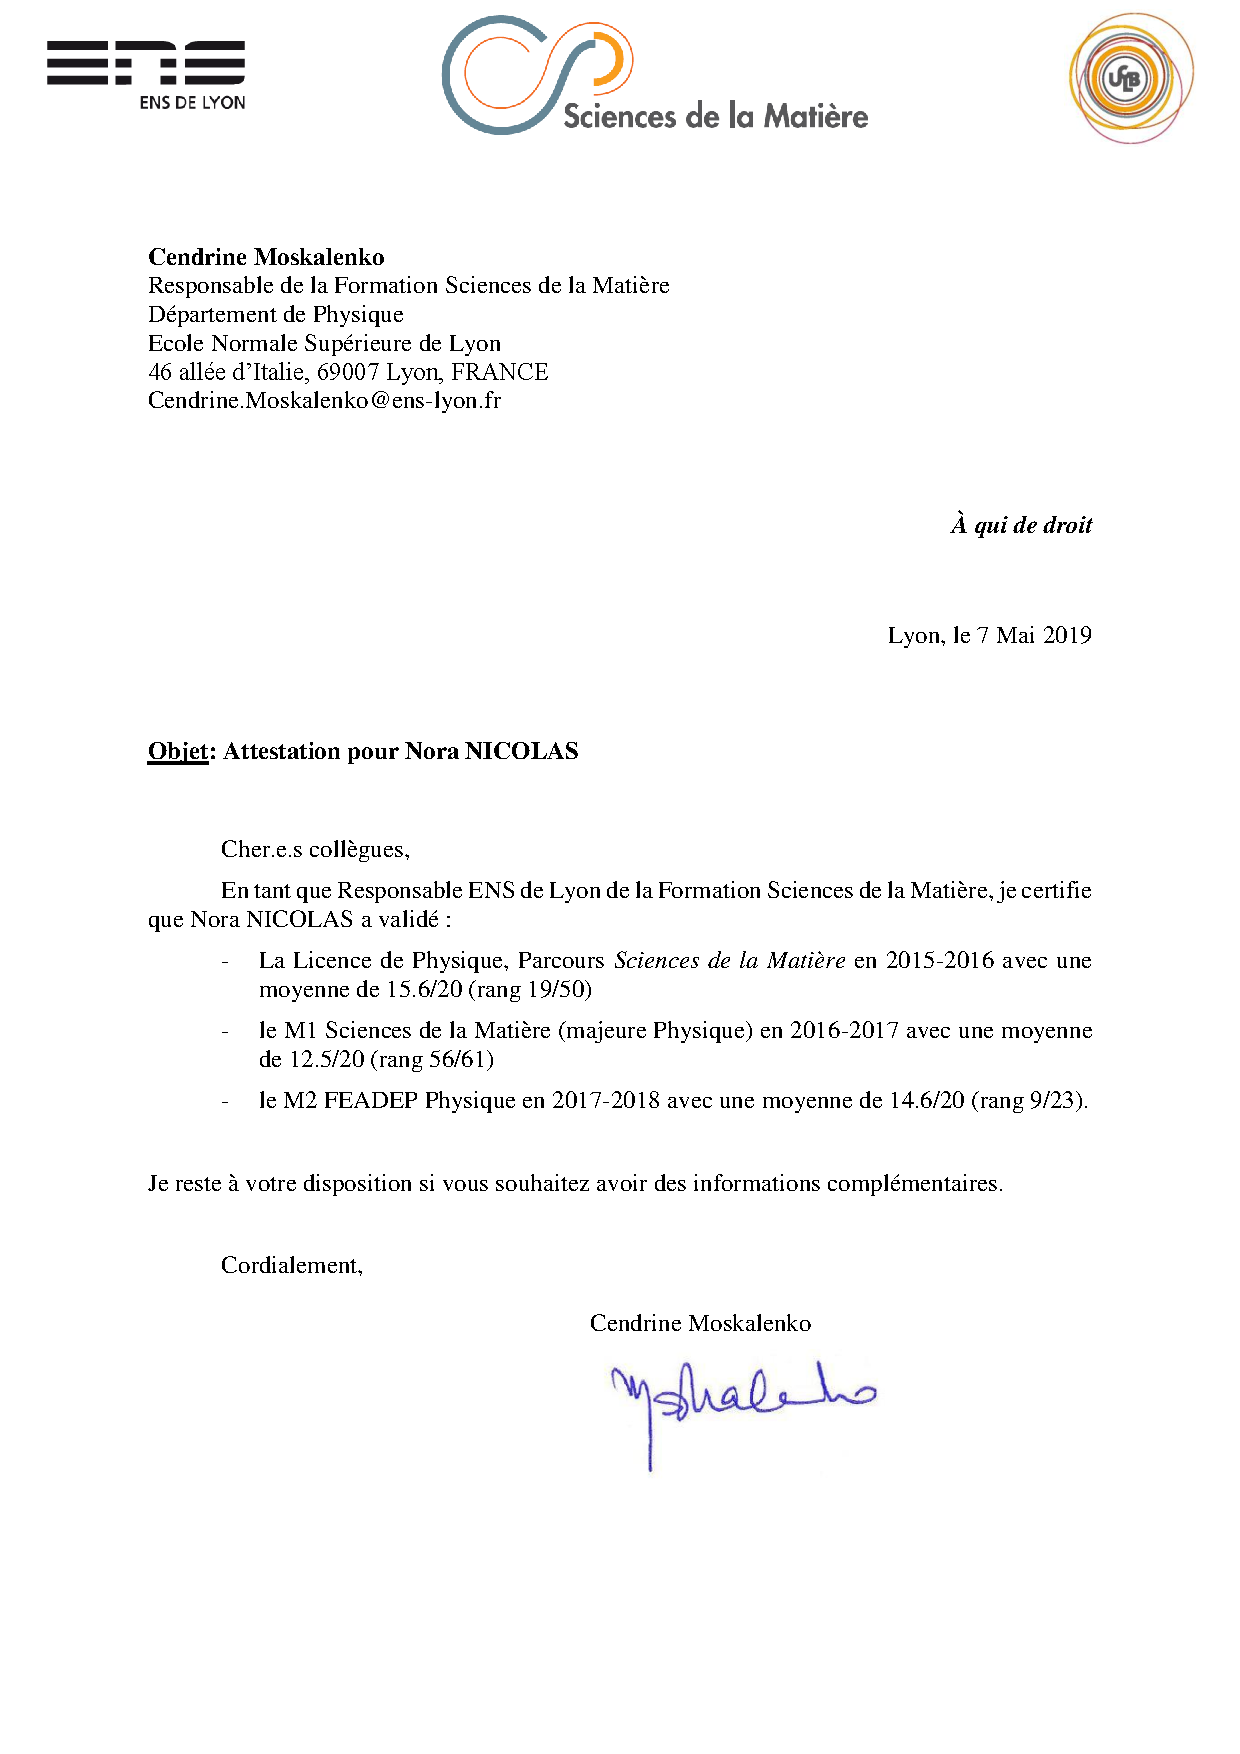
\includepdf[pages=-]{attestation.pdf}
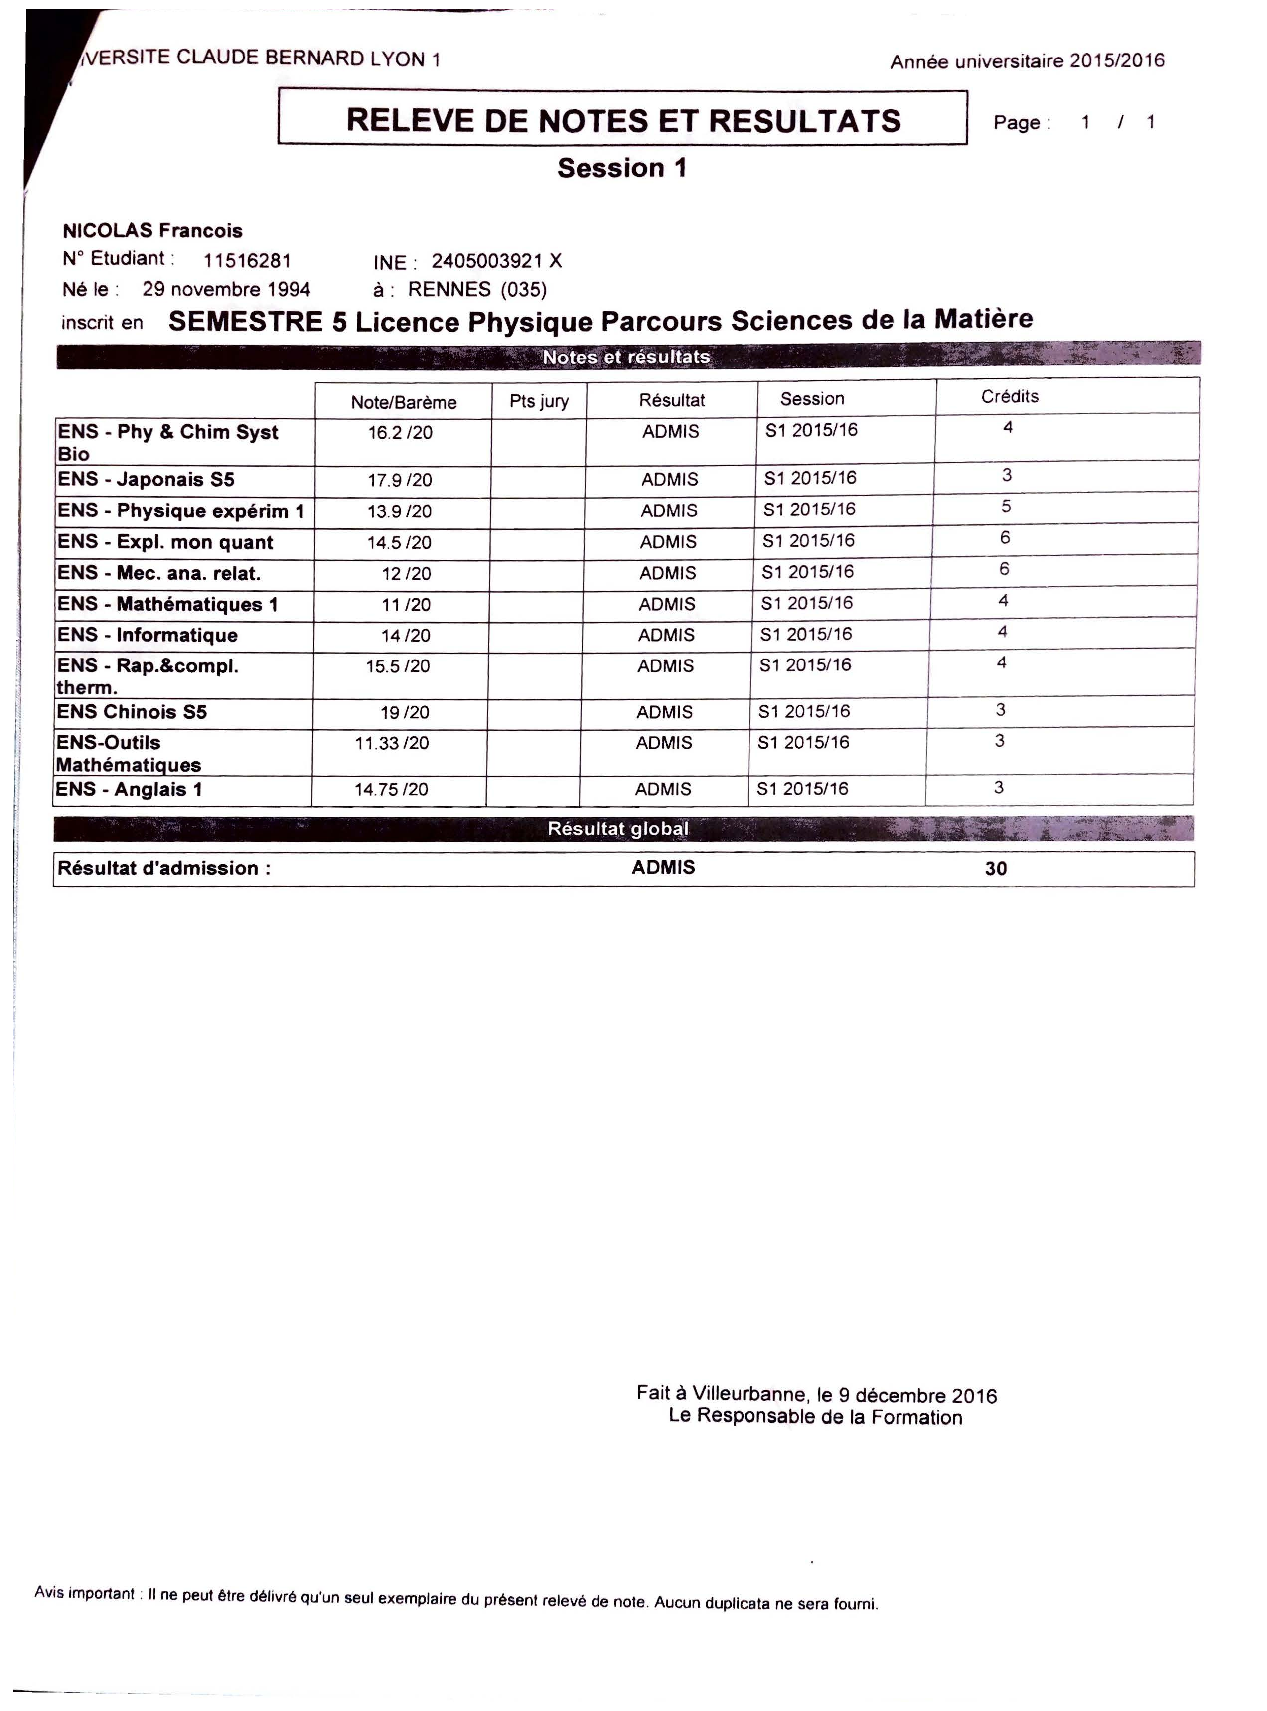
\includepdf[pages=-]{notes_L3.pdf}
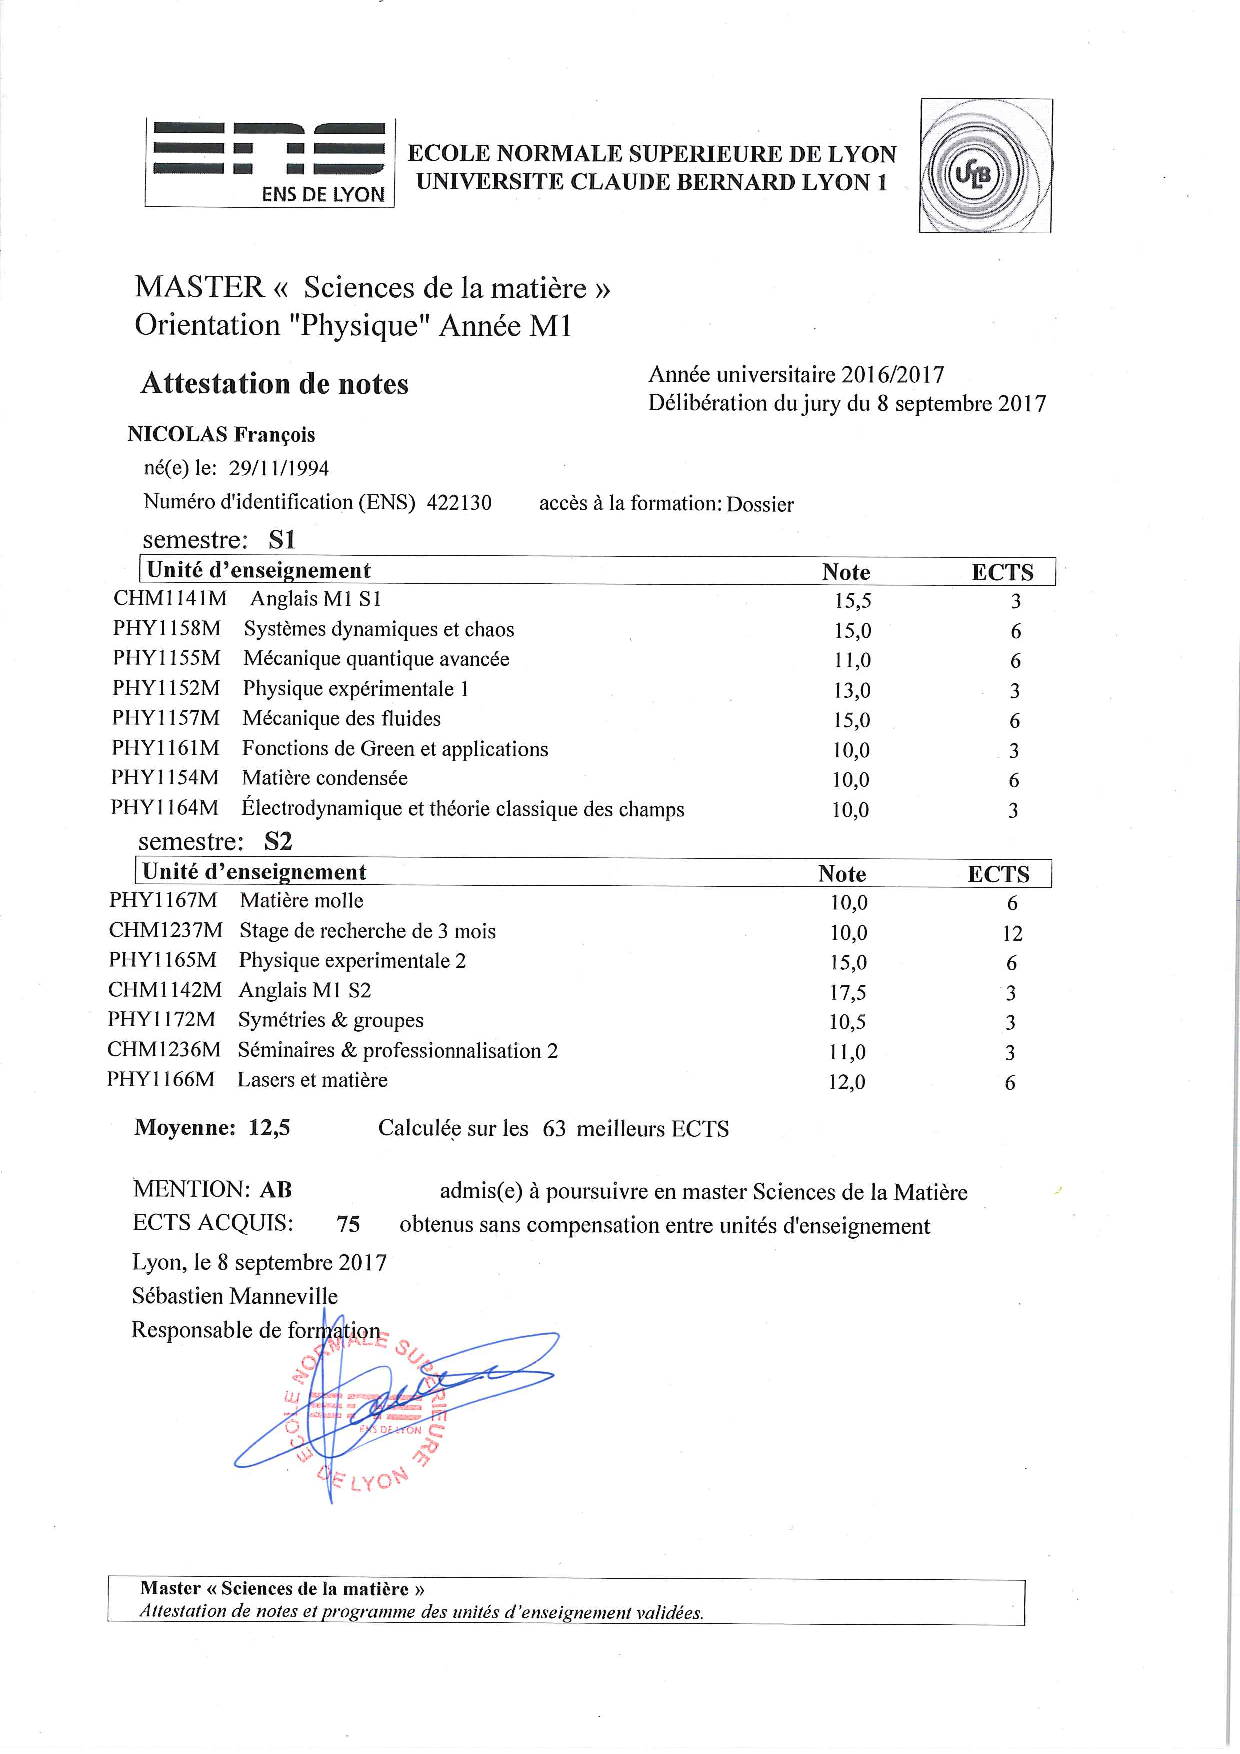
\includepdf[pages=-]{notes_M1.pdf}
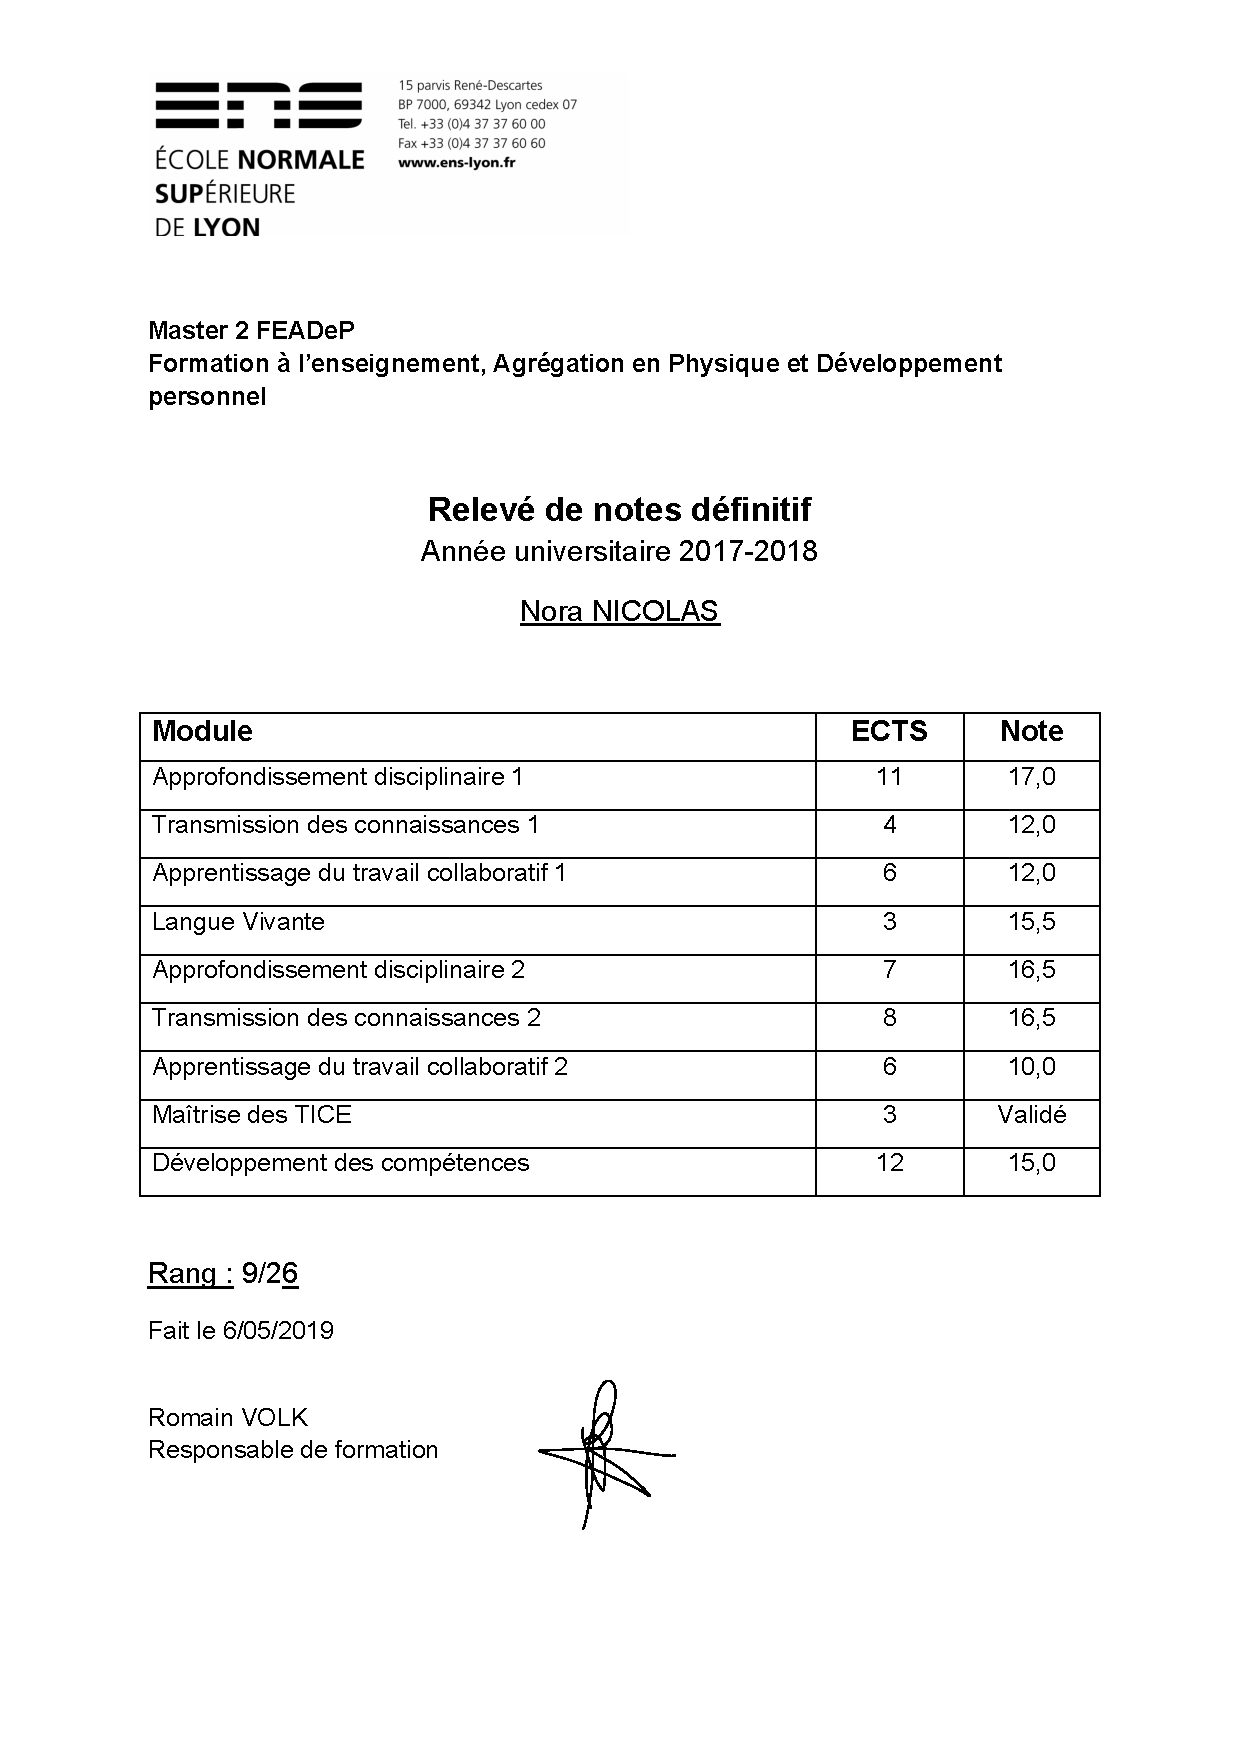
\includepdf[pages=-]{notes_agreg.pdf}
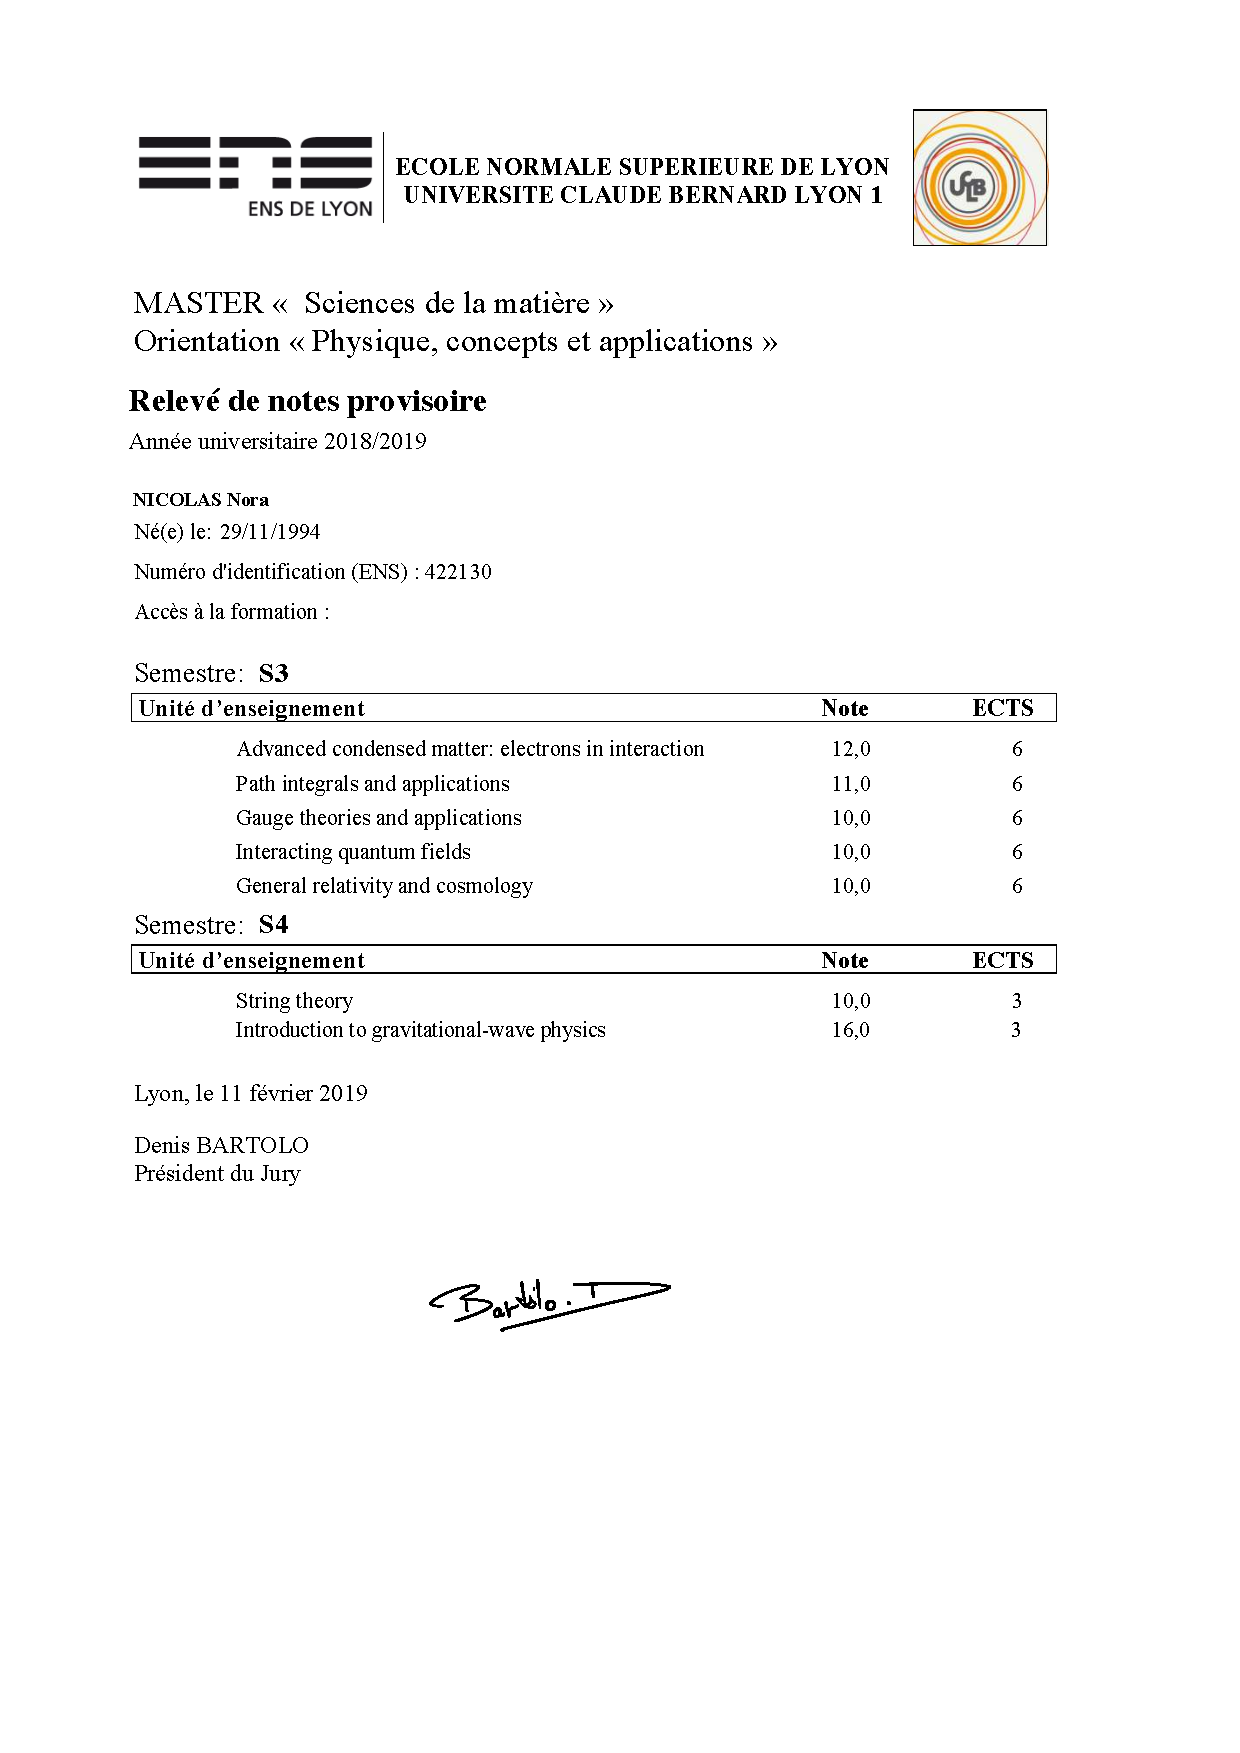
\includepdf[pages=-]{notes_M2.pdf}
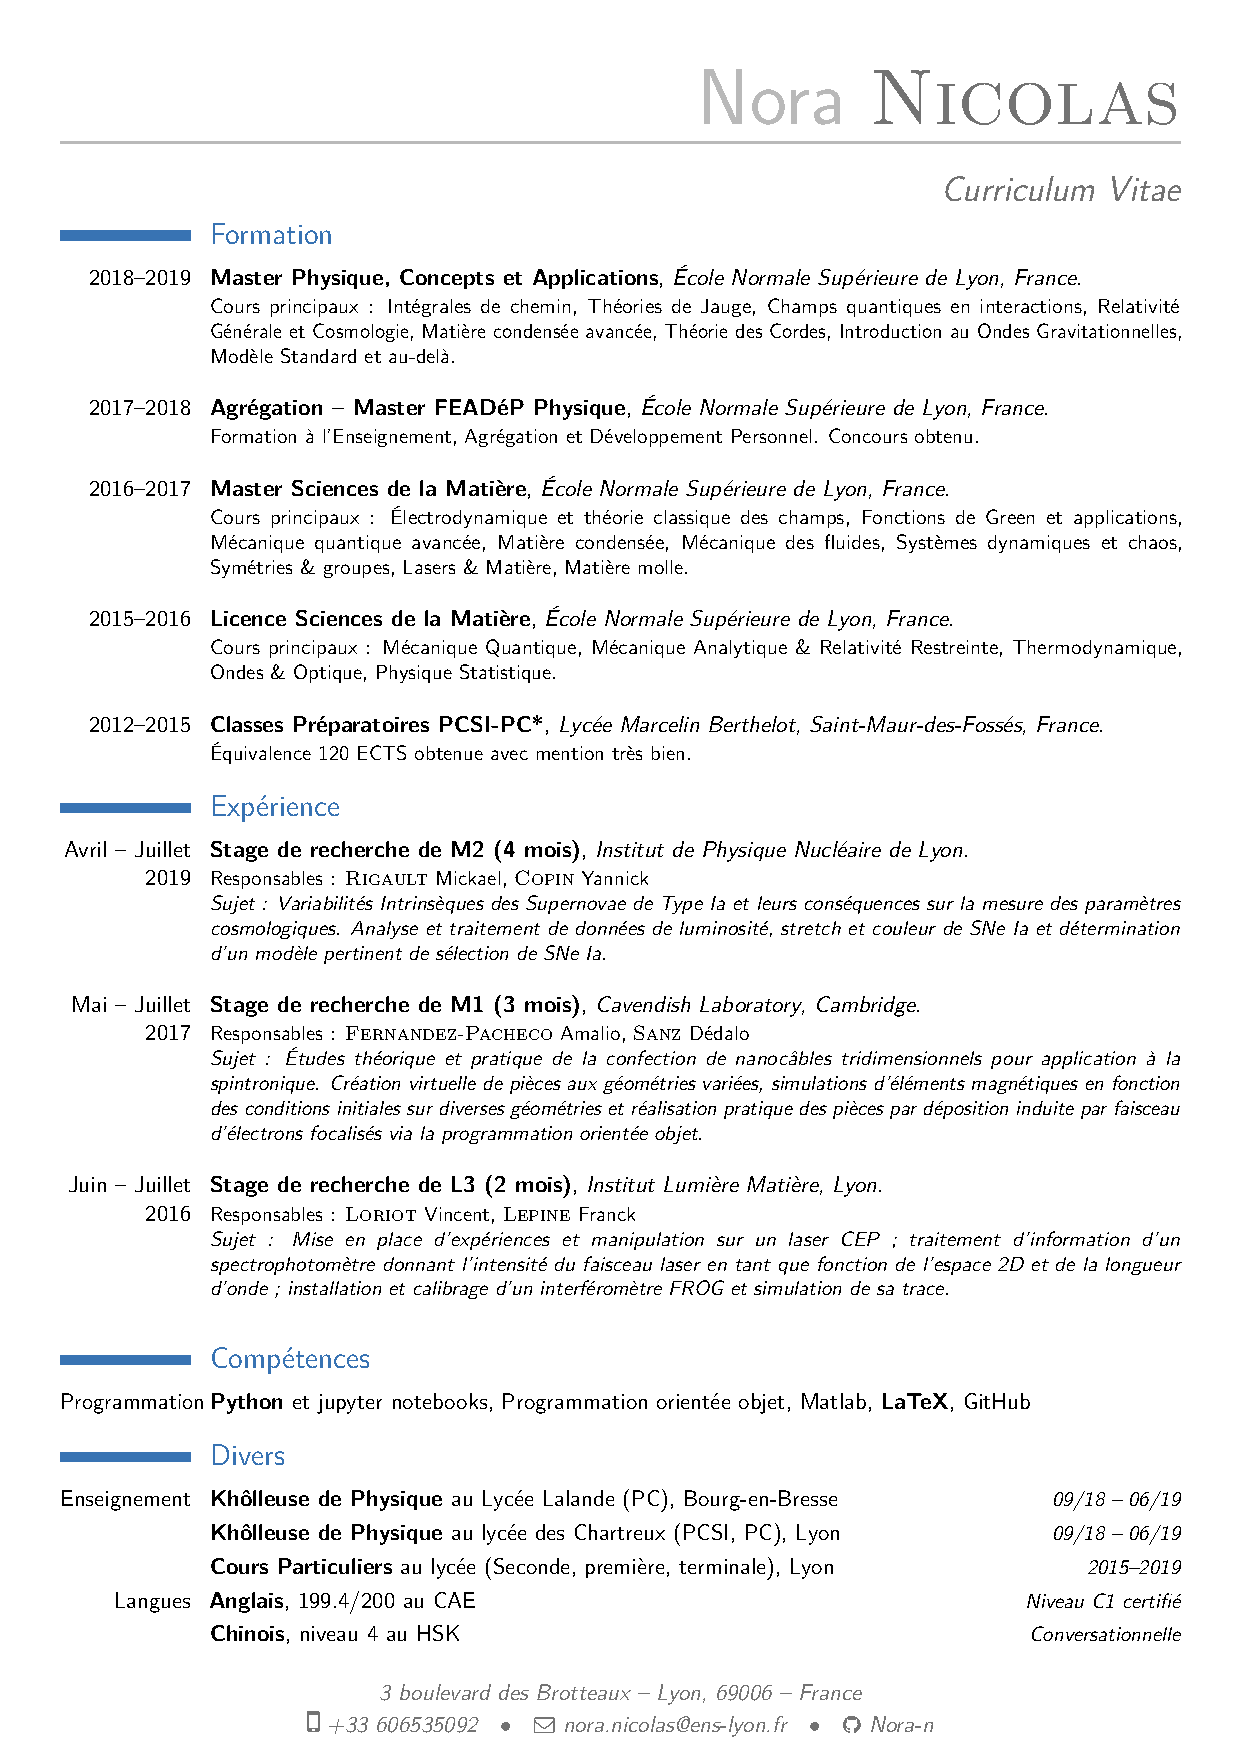
\includepdf[pages=-]{CV/CV_Nora_NICOLAS_2019_French.pdf}

\end{document}
